
\providecommand{\myrootdir}{..}
\documentclass[\myrootdir/main.tex]{subfiles}

\begin{document}

\chapter{Information Extraction Tool}
\label{sec:implementation}
We implemented prototypes for our three focus information extraction techniques to evaluate them on our collected build logs.
This section will present our unified interface and describe the implementation of each of the techniques.


\begin{figure}[h]
	\centering
	\includegraphics[page=7, width=\textwidth, trim={0.5cm 0.5cm 0.5cm 0.5cm}, clip]{img/flow-of-research.pdf}
	\caption{Our tool unifying different information extraction techniques for build logs}
	\label{fig:tool}
\end{figure}

\section{Common Interface}
\begin{lstlisting}
Usage: ruby run-extraction.rb -a analyze -t <technique: ir, pbe, random> -e <example_set> -p <path_to_file_to_analyze>
       ruby run-extraction.rb -a evaluate -t <technique: ir, pbe, keyword, random> -e <example_set> -s <selection_technique> -l <step_count_for_learning> -c <test_count>
       ruby run-extraction.rb -a analyze -t keyword -k <keyword, keyword, ...> -p <path_to_file_to_analyze>
       ruby run-extraction.rb -a analyze -t regex -r <regex to match extraction> -p <path_to_file_to_analyze>

Specific options:
    -a, --action ACTION              Either run an extraction for a example set ('analyze') or run the whole evaluation of it ('evaluate')
    -t, --technique TECHNIQUE        The technique used for creating the extraction program (pbe, ir, keyword, random)
    -e, --example-set EXAMPLE_SET    The filename of the example set to use
    -p, --path PATH                  The path to the file to be analyzed relative to the 'tool/samples' folder
    -s, --selection SELECTION        The example sequence selection technique to use for evaluation (chronological, random, manual (= like defined in file))
    -l, --learning-step-count COUNT  How many steps with increasing example set size to do during evaluation
    -c, --test-count COUNT           How many test files to evaluate the generated program in each learning step of the evaluation
    -v, --verbose                    Print additional interesting output apart from only the extraction output
    -k, --keywords X,Y,Z             Keywords too filter lines for during keyword search based extraction
    -r, --regex REGEX                Regex to match on build log file content in regex based extraction

Common options:
    -h, --help                       Show this message
\end{lstlisting}
As we implemented the information extraction techniques in different languages, choosing one that fits the respective technique each time, we decided to abstract over language differences for cli arguments by creating a unified interfaces. Our unified interface then in turn calls the various different IE techniques over the command line.

We provide two different modes: \emph{analysis} and \emph{evaluation}.
The \emph{analysis} takes a path to a file you want to analyze and all the configuration necessary for a specific technique and returns the resulting extraction on the console output. The \emph{evaluation} takes an 

unification tool, reference CLI somehow nicely?,

ruby tool, unifies different syntax command line interfaces of the other tools, easy to switch between different techniques (NOT TOO LONG)

\section{Overall Implementation Remarks}
There are multiple implementation specialities that span over all languages, frameworks and implemented techniques.
The following section discusses preprocessing and escaping of the parsed build log files / example sets, as well as ... \todo{more?}

\subsection{Preprocessing Log Text}
\label{sec:impl-preprocessing}

\section{PROSE Program Synthesis}
\label{sec:impl-pbe}
The first technique we implemented was the PROSE regular expression program synthesis. As it is based on the PROSE library from Microsoft provided in C\# we also chose C\# for our tool. 
implementation details :)

C\#, based on PROSE Text Extraction DSL, parsing example set files, feeding learning session \& applying learned regex program, can do single string extraction and also sequence extraction \& showing differentiating examples (although not in use)

\section{IR Similarity}
impl details,

R, text2vec, tokenized vectors, impl of preprocessing?

don't repeat from IE models section!

\section{Keyword search}
impl details,

R, simple!

\end{document}
